% ================================================================
%  CAPITOLO 2 - PULSANTE
% ================================================================
\chapter{Pulsante}

% ----------------------------------------------------------------
\section{Introduzione}

\begin{minipage}[c]{0.48\textwidth}
    Il \textbf{pulsante} (o \textit{push button}) è uno dei componenti di input più semplici e comuni nel mondo dell'elettronica. Viene utilizzato per inviare un comando dall'utente al sistema: può accendere o spegnere una luce, avviare un processo, selezionare un'opzione e molto altro. Lo troviamo quotidianamente su telecomandi, tastiere, suonerie di campanelli, pulsanti di accensione e innumerevoli altre applicazioni.
\end{minipage}%
\hfill
\begin{minipage}[c]{0.48\textwidth}
    \centering
    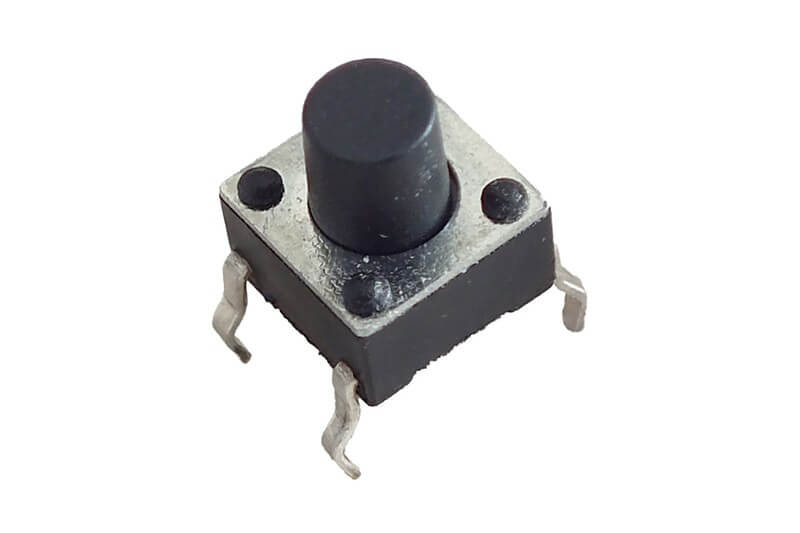
\includegraphics[width=0.4\textwidth]{img/micro-pulsante.jpg}
    \captionof{figure}{Classico pulsante a 4 pin.}
    \label{fig:pulsante}
\end{minipage}

\vspace{0.2cm}
In questo capitolo impareremo come collegare correttamente un pulsante ad Arduino e come scrivere il codice per leggere il suo stato (premuto o rilasciato), gestendo il fenomeno del \textit{rimbalzo} meccanico dei contatti (\textit{bouncing}).

% ----------------------------------------------------------------
\section{Struttura e funzionamento}
% ----------------------------------------------------------------

\subsection*{Come è fatto un pulsante}

Un pulsante è un interruttore momentaneo: quando viene premuto, chiude un circuito elettrico; quando viene rilasciato, lo riapre. La struttura interna più semplice è composta da quattro terminali (pin). In realtà, i terminali sono collegati a coppie: due terminali sono sempre connessi tra loro internamente, e gli altri due sono sempre connessi tra loro. Quando si preme il pulsante, le due coppie si collegano, chiudendo il circuito.

    
\begin{figure}[h]
    \centering
    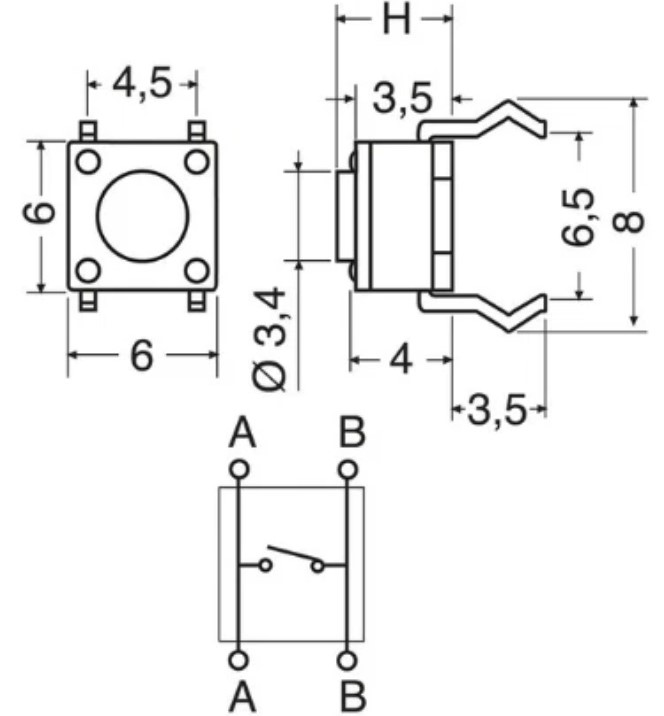
\includegraphics[width=0.3\textwidth]{img/struttura interna pulsante.jpg}
    \caption{Struttura interna di un pulsante a 4 pin.}
    \label{fig:interno_pulsante}
\end{figure}


I pulsanti utilizzati nei kit didattici hanno spesso quattro piedini disposti su due lati. I due piedini sullo stesso lato sono internamente collegati. Quindi, per collegare un pulsante ad Arduino, è sufficiente utilizzare un piedino da ciascuna coppia, ad esempio uno del lato A e uno del lato B. In questo modo, quando si preme il pulsante, si chiude il circuito tra i due piedini utilizzati.

\subsection*{Stati del pulsante}

Dal punto di vista elettrico, un pulsante può trovarsi in due stati:
\begin{itemize}
    \item \textbf{Aperto (rilasciato)}: i contatti interni non si toccano, il circuito è aperto e non scorre corrente.
    \item \textbf{Chiuso (premuto)}: i contatti interni si toccano, il circuito è chiuso e la corrente può scorrere.
\end{itemize}

\begin{tcolorbox}[colback=blue!4, colframe=blue!60, title=\textbf{Esercizi proposti}]
    \begin{enumerate}
        \item \textbf{Continuità:} Utilizzando un multimetro in modalità di continuità, misurare la resistenza tra i pin del pulsante quando è premuto e quando è rilasciato.
        \item \textbf{Circuito con LED: } Collegare un LED e una resistenza in serie al pulsante, alimentandolo con un generatore impostato a \SI{9}{\volt}. Verificare che il LED si accenda solo quando il pulsante è premuto.
    \end{enumerate}
\end{tcolorbox}
% ----------------------------------------------------------------
\section{Arduino e resistenze di pull-up e pull-down}
% ----------------------------------------------------------------

\subsection*{Perché sono necessarie}

Un pin di ingresso digitale di Arduino deve sempre vedere una tensione ben definita: \texttt{HIGH} (vicino a \SI{5}{\volt}) o \texttt{LOW} (vicino a \SI{0}{\volt}). Se il pin non è collegato a nulla (floating), può captare disturbi elettromagnetici e leggere valori casuali. La resistenza di \textit{pull-up} o \textit{pull-down} fissa il pin a uno stato logico noto quando il pulsante non è premuto.

\subsection*{Configurazione pull-down}

Nel circuito \textbf{pull-down}, il pin di ingresso è collegato a massa (GND) tramite una resistenza di alto valore (tipicamente \SI{10}{\kilo\ohm}). Il pulsante collega il pin a \SI{5}{\volt} quando viene premuto.

\begin{figure}[h]
    \centering
    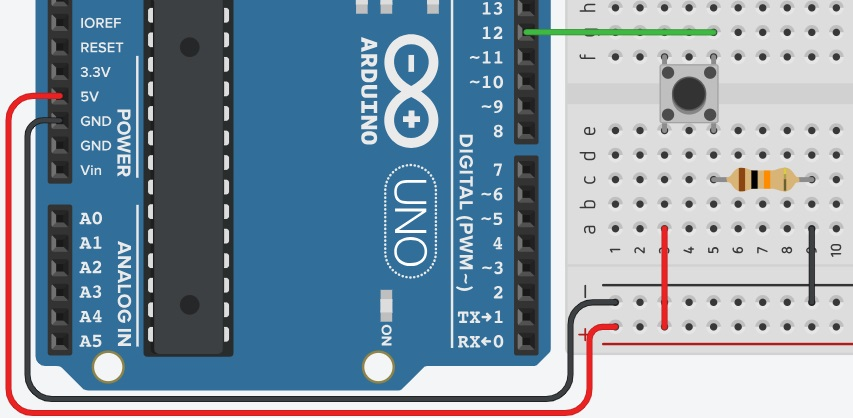
\includegraphics[width=0.84\textwidth]{img/Pull-Down.jpg}
    \caption{Collegamento pull-down: pin LOW a riposo, HIGH quando premuto.}
    \label{fig:pull_down}
\end{figure}

\begin{itemize}
    \item \textbf{Pulsante non premuto}: il pin è collegato a GND tramite la resistenza → legge \texttt{LOW}.
    \item \textbf{Pulsante premuto}: il pin è collegato direttamente a \SI{5}{\volt} (la resistenza è in parallelo ma la corrente preferisce il percorso a bassa resistenza del pulsante) → legge \texttt{HIGH}.
\end{itemize}

\subsection*{Configurazione pull-up}

Nel circuito \textbf{pull-up}, il pin di ingresso è collegato a \SI{5}{\volt} tramite una resistenza. Il pulsante collega il pin a GND quando viene premuto.

\begin{figure}[h]
    \centering
    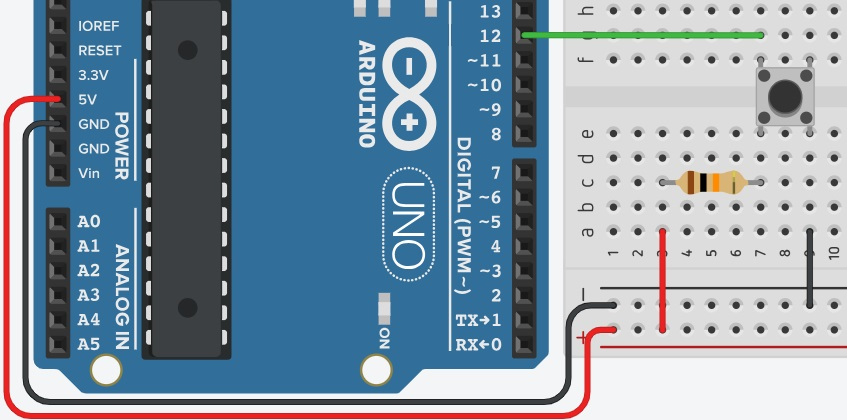
\includegraphics[width=0.67\textwidth]{img/Pull-Up.jpg}
    \caption{Collegamento pull-up: pin HIGH a riposo, LOW quando premuto.}
    \label{fig:pull_up}
\end{figure}

\begin{itemize}
    \item \textbf{Pulsante non premuto}: il pin è collegato a \SI{5}{\volt} tramite la resistenza → legge \texttt{HIGH}.
    \item \textbf{Pulsante premuto}: il pin è collegato direttamente a GND → legge \texttt{LOW}.
\end{itemize}

\begin{tcolorbox}[colback=red!4, colframe=red!60, title=\textbf{Attenzione: importanza del resistore}]
    Non collegare un pulsante direttamente tra \SI{5}{\volt} e GND \textbf{senza una resistenza}, altrimenti si crea un cortocircuito quando il pulsante è premuto, che può danneggiare Arduino.
\end{tcolorbox}

\subsection{Pull-Up interno ad arduino}
Sui pin digitali di Arduino è possibile attivare una resistenza di pull-up interna, evitando di doverla collegare esternamente. Per farlo, basta configurare il pin come \texttt{INPUT\_PULLUP} nel codice. In questo modo, il pin sarà collegato internamente a \SI{5}{\volt} tramite una resistenza di pull-up, e il pulsante dovrà collegare il pin a GND per essere letto come \texttt{LOW} quando premuto.

\begin{figure}[h]
    \centering
    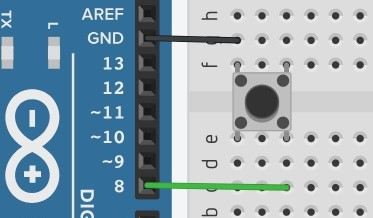
\includegraphics[width=0.55\textwidth]{img/Pull-Up_Interno.jpg}
    \caption{Collegamento pull-up interno ad Arduino}
    \label{fig:pull_up_interno}
\end{figure}

\section{Programmazione con Arduino}
% ----------------------------------------------------------------

\subsection*{Leggere lo stato del pulsante: \texttt{digitalRead()}}

Per leggere il valore logico presente su un pin digitale si usa la funzione \texttt{digitalRead()}, che restituisce \texttt{HIGH} o \texttt{LOW}.

\begin{center}
    \hrule
    \vspace{0.2cm}
    \texttt{int valore = digitalRead(numeroPIN);}
    \vspace{0.2cm}
    \hrule
\end{center}

Il valore restituito è \texttt{HIGH} se sul pin è presente una tensione di circa \SI{5}{\volt}, altrimenti se la tensione è vicina a \SI{0}{\volt} allora verrà restituito \texttt{LOW}.

\subsection*{Leggere e stampare sul seriale}

Colleghiamo il pulsante al pin 2 con pull-up interno e inviamo lo stato al monitor seriale.

\begin{tcblisting}{
    listing only,
    listing engine=listings,
    colback=teal!5,
    colframe=teal!50,
    title=\textbf{Esempio 1 - Lettura semplice},
    breakable,
    listing options={
        language=C++,
        basicstyle=\ttfamily\small,
        keywordstyle=\color{blue!80!black}\bfseries,
        commentstyle=\color{green!50!black}\itshape,
        stringstyle=\color{orange!80!black},
        numbers=left,
        numberstyle=\tiny\color{gray},
        breaklines=true,
        showstringspaces=false,
        morekeywords={pinMode, digitalRead, digitalWrite, Serial, begin, println, INPUT\_PULLUP, HIGH, LOW, void, const, int, if, else}
    }
}
// Pin a cui è collegato il pulsante
const int buttonPin = 2;
// Variabile per memorizzare lo stato   
bool buttonState = LOW;    

void setup() {
    Serial.begin(9600);                
    pinMode(buttonPin, INPUT_PULLUP);  // Pin con pull-up interno
}

void loop() {
    // Legge stato pulsante
    buttonState = digitalRead(buttonPin);

    // se lo stato è uguale a LOW, vuol dire che è stato premuto
    if (buttonState == LOW) {              
        Serial.println("Pulsante premuto");
    } else {
        Serial.println("Pulsante rilasciato");
    }

    // Piccola pausa per evitare troppi messaggi
    delay(50);
}
\end{tcblisting}

\section{Il problema del rimbalzo - Bouncing}

Creiamo un codice per contare quante volte il pulsante viene premuto. L'idea è semplice: ogni volta che rileviamo una transizione da \texttt{HIGH} a \texttt{LOW} (pulsante premuto), incrementa un contatore.

\begin{tcblisting}{
    listing only,
    listing engine=listings,
    colback=teal!5,
    colframe=teal!50,
    title=\textbf{Esempio 2 - Contatore pressioni},
    breakable,
    listing options={
        language=C++,
        basicstyle=\ttfamily\small,
        keywordstyle=\color{blue!80!black}\bfseries,
        commentstyle=\color{green!50!black}\itshape,
        stringstyle=\color{orange!80!black},
        numbers=left,
        numberstyle=\tiny\color{gray},
        breaklines=true,
        showstringspaces=false,
        morekeywords={pinMode, digitalRead, digitalWrite, Serial, begin, println, INPUT\_PULLUP, HIGH, LOW, void, const, int, if, else}
    }
}
const int buttonPin = 2;      // Pin a cui è collegato il pulsante
bool stato_attuale = HIGH;    // Memorizza lo stato attuale
bool stato_precedente = HIGH; // Memorizza lo stato precedente
int contatore = 0;            // Contatore di pressioni

void setup() {
    Serial.begin(9600);                
    pinMode(buttonPin, INPUT_PULLUP);  // Pin con pull-up interno
}

void loop() {
    // Legge stato pulsante
    stato_attuale = digitalRead(buttonPin);

    // se lo stato è cambiato, vuol dire che è stato premuto
    if (stato_attuale == LOW && stato_precedente == HIGH) {              
        contatore++;
        Serial.print("Pulsante premuto ");
        Serial.print(contatore);
        Serial.println(" volte");
    }

    // Aggiorna stato precedente
    stato_precedente = stato_attuale; 
}
\end{tcblisting}

\begin{tcolorbox}[colback=red!4, colframe=red!60, title=\textbf{Attenzione: il risultato non è quello atteso!}]

    Proviamo adesso a premere il pulsante esattamente 30 volte. Se tutto funziona correttamente, l'ultima stampa dovrebbe essere "Pulsante premuto 30 volte" sul monitor seriale. Tuttavia potremmo vedere un numero più alto di 30 anche se abbiamo premuto il pulsante solo 30 volte.
\end{tcolorbox}

Quando il pulsante viene premuto o rilasciato, i contatti meccanici non si chiudono o aprono in modo pulito: rimbalzano per alcuni millisecondi (tipicamente 5–20 ms), generando una rapida sequenza di transizioni HIGH-LOW-HIGH. Arduino legge questi rimbalzi come molte pressioni anziché una sola.

\begin{figure}[h]
    \centering
    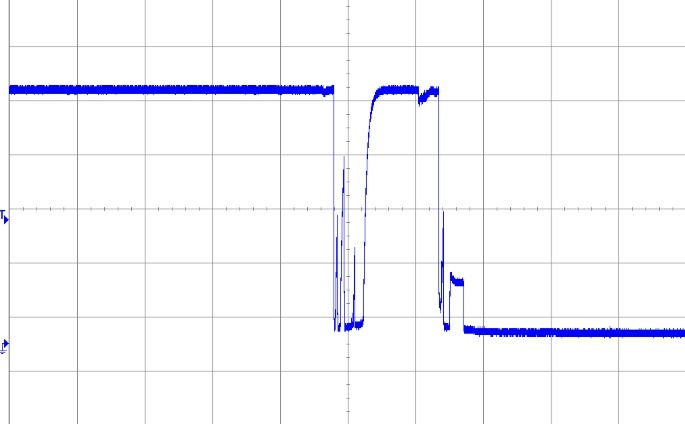
\includegraphics[width=0.8\textwidth]{img/bouncing.jpg}
    \caption{Rappresentazione del rimbalzo meccanico dei contatti di un pulsante.}
    \label{fig:bouncing}
\end{figure}

\subsection*{Soluzione al problema del bouncing: Bounce2}

Esiste una libreria chiamata \textbf{Bounce2} che implementa un algoritmo di debouncing efficace. La libreria filtra i rimbalzi e fornisce metodi per rilevare quando il pulsante è stato effettivamente premuto o rilasciato.

Per installare la libreria Bounce2, apri l'IDE di Arduino, nel menù a sinistra c'è un'icona con dei libri (Gestore librerie). Cliccaci sopra, poi nella barra di ricerca scrivi "Bounce2" e installa la libreria sviluppata da Thomas Ouellet Fredericks.

Questa libreria utilizza un approccio basato su timer per ignorare i rimbalzi. Quando viene rilevata una transizione, la libreria aspetta un intervallo di tempo predefinito (ad esempio 50 ms) prima di considerare la transizione come valida. Se durante questo intervallo si verificano altre transizioni, vengono ignorate.


Vediamo un esempio di utilizzo della libreria Bounce2 per contare le pressioni di un pulsante senza essere influenzati dai rimbalzi.

\begin{tcblisting}{
    listing only,
    listing engine=listings,
    colback=teal!5,
    colframe=teal!50,
    title=\textbf{Esempio - Utilizzo libreria Bounce2 con pulsante},
    breakable,
    listing options={
        language=C++,
        basicstyle=\ttfamily\small,
        keywordstyle=\color{blue!80!black}\bfseries,
        commentstyle=\color{green!50!black}\itshape,
        stringstyle=\color{orange!80!black},
        numbers=left,
        numberstyle=\tiny\color{gray},
        breaklines=true,
        showstringspaces=false,
    }
}
// Libreria per eliminare i rimbalzi del pulsante
#include <Bounce2.h>   

const int buttonPin = 2;
int contatore = 0;

// Oggetto che gestisce il pulsante con filtro anti-rimbalzo
Bounce debouncer = Bounce(); 

void setup() {
    pinMode(buttonPin, INPUT_PULLUP);
    Serial.begin(9600);

    // Colleghiamo la libreria al pin del pulsante
    debouncer.attach(buttonPin);  

    // Impostiamo 50 ms come tempo di stabilizzazione del segnale
    debouncer.interval(50);  
    
}

void loop() {
    // Aggiorna continuamente lo stato del pulsante 
    debouncer.update();  

    // Se pulsante è stato premuto, stampa il contatore aggiornato
    if (debouncer.fell()) {
        contatore++;
        Serial.println(contatore);
    }
}
\end{tcblisting}

La libreria utilizzata risolve questo problema controllando il segnale nel tempo: quando rileva un cambiamento, aspetta che il segnale si stabilizzi per un breve intervallo (in questo caso 50 millisecondi). Solo dopo questo controllo considera la pressione valida.
Nel programma, ogni volta che viene rilevata una pressione reale del pulsante, viene aumentata di uno una variabile chiamata contatore. In questo modo si può sapere quante volte il pulsante è stato premuto in modo affidabile.

\subsection*{Funzioni importanti della libreria Bounce2 DA MODIFICARE}
La libreria \textbf{Bounce2} permette di gestire in modo affidabile i pulsanti eliminando i problemi causati dai rimbalzi elettrici. Tra i metodi più importanti c’è \texttt{attach()}, che serve a collegare la libreria a un determinato pin e a impostarne la modalità di funzionamento (come ingresso normale o con resistenza di pull-up). Un altro metodo fondamentale è \texttt{update()}, che deve essere chiamato continuamente nel ciclo principale del programma per aggiornare lo stato del pulsante e applicare il filtro anti-rimbalzo.

Per definire il tempo di stabilizzazione del segnale si utilizza \texttt{interval()}, che imposta per quanti millisecondi il segnale deve restare stabile prima di essere considerato valido. Per sapere se il pulsante è premuto in un determinato momento si può usare \texttt{isPressed()}, mentre \texttt{pressed()} e \texttt{released()} servono per rilevare rispettivamente l’istante in cui il pulsante viene premuto o rilasciato.

Molto utili sono anche \texttt{fell()} e \texttt{rose()}, che permettono di rilevare le transizioni del segnale: \texttt{fell()} indica il passaggio da alto a basso (tipico di una pressione con pull-up), mentre \texttt{rose()} indica il passaggio da basso ad alto. Infine, metodi come \texttt{changed()} permettono di sapere se lo stato del pulsante è cambiato dall’ultimo aggiornamento, mentre \texttt{read()} restituisce semplicemente lo stato attuale del pin.

\subsection*{Rilevare la durata della pressione}

Possiamo misurare per quanto tempo il pulsante rimane premuto usando \texttt{millis()}.

\begin{tcblisting}{
    listing only,
    listing engine=listings,
    colback=teal!5,
    colframe=teal!50,
    title=\textbf{Esempio 4 - Durata pressione},
    breakable,
    listing options={
        language=C++,
        basicstyle=\ttfamily\small,
        keywordstyle=\color{blue!80!black}\bfseries,
        commentstyle=\color{green!50!black}\itshape,
        stringstyle=\color{orange!80!black},
        numbers=left,
        numberstyle=\tiny\color{gray},
        breaklines=true,
        showstringspaces=false,
    }
}
const int buttonPin = 2;
unsigned long pressStart = 0;
bool wasPressed = false;

void setup() {
    Serial.begin(9600);
    pinMode(buttonPin, INPUT_PULLUP);
}

void loop() {
    bool isPressed = (digitalRead(buttonPin) == LOW);
    
    if (isPressed && !wasPressed) {
        pressStart = millis();          // inizio pressione
        wasPressed = true;
    }
    else if (!isPressed && wasPressed) {
        unsigned long duration = millis() - pressStart;
        Serial.print("Pulsante premuto per ");
        Serial.print(duration);
        Serial.println(" ms");
        wasPressed = false;
    }
    delay(10);
}
\end{tcblisting}

\begin{tcolorbox}[colback=red!4, colframe=red!60, title=\textbf{Attenzione: delay() blocca il programma}]
    L'uso di \texttt{delay()} per il debouncing blocca l'esecuzione del programma, impedendo di leggere altri sensori o eseguire azioni contemporanee. Per applicazioni più avanzate, utilizzare tecniche non bloccanti basate su \texttt{millis()}.
\end{tcolorbox}


